\Subsubsubsection{Cálculo Potencias}
Se asumen las siguientes variables para los cálculos de potencias, obtenidas de estadísticas propias de la zona donde se realiza el estudio \cite{ref:weather_bariloche}.
\begin{enumerate}
	\item Duración noche = 12.8 horas.
	\item Duración día = 11.2 horas.
	\item Horas de sol efectivas = 8 horas.
\end{enumerate}

Para el caso de la \rpi, se tiene que su consumo mínimo normal es de $P_{rpi_{min}} = 1.2 \ W$. Sin embargo, para reducir este consumo, se desactivan los puertos de Ethernet y HDMI ya que no se utilizará un entorno gráfico. Esto permite reducir aún más el consumo mínimo. Se estima que la \rspi consumirá como máximo alrededor de $P_{rpi_{est}} = 1.75 \ W$ en su funcionamiento normal \cite{ref:pot_rpi}. Luego, se tiene que el consumo energético por día será de
\begin{equation}
	E_{sist} = P_{rpi_{est}}\cdot 24 \ hs = 151.2 \ kJ
\end{equation}

Teniendo en cuenta que la batería tiene una tensión de $V_{bat} = 12 \ V$ debe tener una capacidad de almacenamiento equivalente a $T_{reserva} = 4 \ d\acute{\imath}as$ sin recarga \cite{ref:weather_bariloche} y utilizando un coeficiente de seguridad de $\gamma_{bat} = 1.5$, se obtiene
\begin{equation}
	Capacidad_{bat} = \frac{E_{sist}\cdot T_{reserva}\cdot 1000}{V_{bat}\cdot 3600}\cdot \gamma_{bat} = 21 \ Ah
\end{equation}

Por otro lado, para los cálculos del panel solar, teniendo en cuenta que se quiere que en un día de sol promedio se logre abastecer al sistema de su consumo energético normal diario y recargar un $\rho = 0.2$ de la capacidad total de la batería, y además teniendo en cuenta un coeficiente de seguridad de $\gamma_{panel} = 2$, se tiene que
\begin{equation}
	Pot_{panel} = \left( E_{sist} + \frac{Capacidad_{bat}\cdot V_{bat}\cdot 3600\cdot \rho}{1000}\right)\cdot \gamma_{panel} \cdot  \frac{1000}{60\cdot 60\cdot 8 \ hs} = 23.1 \ W
\end{equation}
\Subsubsubsection{Protección para alimentación \rspi}
Ante la eventual pérdida de energía, en condiciones de funcionamiento normal, es sumamente probable que la memoria SD de la \rspi resulte corrupta, y por consiguiente inutilizable. Esto está contemplado en \textit{T-INT-16}, por lo que se diseña un circuito de detección  de baja batería, que apaga de manera segura la \rspi.
Para esto se agrega una bornera en la cual se conecta directamente la batería, de esta manera se sensa su nivel de tensión y se determina cuando cuenta con un nivel de carga menor al 25$\%$, en consecuencia cambiando el valor del comparador en bajo, el cual se encuentra conectado a un pin tipo GPIO de la \rspi, que ante este cambio ejecuta el comando de apagado.
\begin{figure}[H]
	\centering
    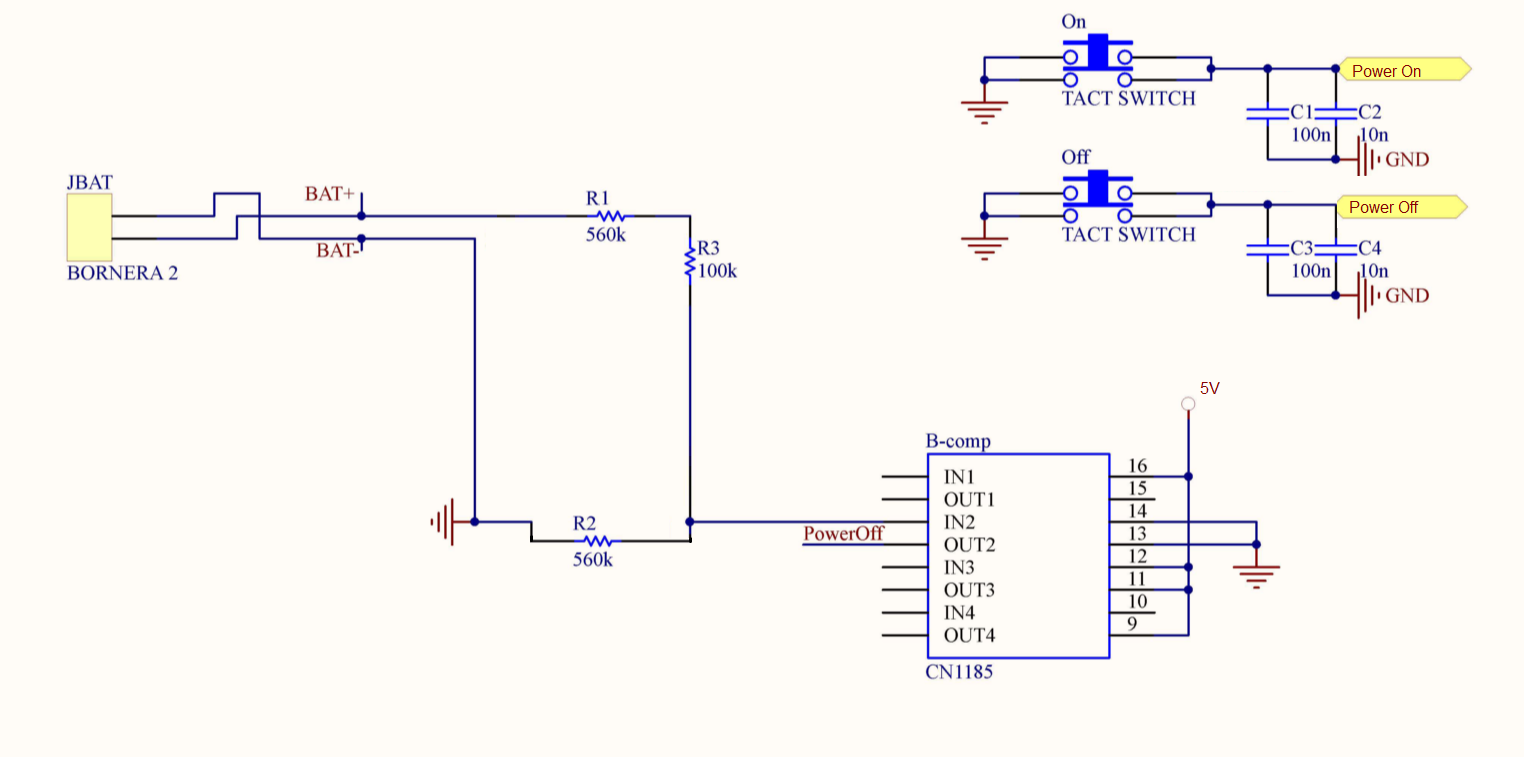
\includegraphics[width=0.7\linewidth]{ImagenesIngenieria de Detalle/Comparador}	
	\caption{Circuito Comparador e interruptores.}
	\label{fig:Comp}
\end{figure}
Adicionalmente se agrega un interruptor para apagado seguro, y uno para prendido seguro, los cuales están destinados para los operarios de instalación y desinstalación, si los necesitasen. 
Finalmente lo último es la configuración de la \rspi para que con el cambio del comparado, se efectúen los cambios.
\begin{lstlisting}[language=bash]
sudo nano /boot/config.txt 
dtoverlay=gpio-shutdown,gpio_pin=26,active_low=1,gpio_pull=up
\end{lstlisting} 
\Subsubsubsection{Cálculo resistencias}

Tanto para el Bus de $I^2C$ como para el DHT22, se calcularon las resistencias de \textit{pull-up}\footnote{En los circuitos digitales, un resistor \textit{pull-up} se utiliza para garantizar que la señal siempre se encuentre en un estado conocido.} de la siguiente manera:
\begin{equation}
	R_p \ = \  \frac{V_{dd}}{I_{R_p}} \ = \ \frac{3.3 \ V}{1 \ mA} \ = \ 3.3 \ k\Omega  
\end{equation}
Para el comparador se toman las especificaciones de la datasheet, para saber cual es la tensión de referencia, y acorde a esta se calcula el divisor resistivo de manera que al tener un nivel de carga menor al 25$\%$ se dispare el comparador.
\begin{equation}
R_1 \ +\ R_2 \ = \ R_a
\end{equation}
\begin{equation}
I_{leak} \ = \ \frac{V_{bat}}{R_a+R_2} 
\end{equation}
\begin{equation}
R_a \ = \ \frac{V_{LowBat} \ \cdot \ R_2}{V_{trigger}} \ - \ R_2
\end{equation}

Con estas ecuaciones se definen los valores de las resistencias.
\begin{equation}
R_1 \ =2.7M\Omega  \ \ R_2 \  = \ 330K\Omega   \ \ R_3 \ = \ 22K\Omega  
\end{equation}

\Subsubsubsection{Cálculo de memoria}
Se definen los siguientes valores para cada medición:
\begin{itemize}
	\item Medición temperatura y humedad: 16 $Bytes$ (fecha y hora) + 4 $Bytes$ (humedad) + 4 $Bytes$ (temperatura) = $24 \ Bytes$.
	\item Medición luminosidad: $16 \ Bytes$ (fecha y hora) + $4 \ Bytes$ (luminosidad) = $20 \ Bytes$.
	\item Medición cámara: cada imagen pesa $1.2 \ MBytes$ \cite{ref:rpicam} (considerando una calidad alta).
	\item Información recibida por BT: aproximadamente $2 \ KByte$.
	\item Sistema operativo: $2 \ GBytes$.
	\item Programas y bibliotecas: $2.8 \ GBytes$.
\end{itemize}

De esta forma se tiene el tamaño de las mediciones durante un período de 14 días:
\begin{multline*}
	12 \ \nicefrac{medici\acute{o}n}{hora} \  \cdot \ 24 \ \nicefrac{hora}{d\acute{\imath}a} \  \cdot \ 14 \ d\acute{\imath}a \  \cdot \ \left( \ 24 \  \nicefrac{Bytes}{medici\acute{o}n} \right. \\ \left. + \ 16 \ \nicefrac{Bytes}{medici\acute{o}n} \ + \ 1.2 \ MBytes \right) \ + 2 \ \nicefrac{KByte}{d\acute{\imath}a} \  \cdot \  14 \ d\acute{\imath}a = 4.84 \ GBy
\end{multline*}

Si a esto se le suma el espacio dedicado al sistema operativo, programas y bibliotecas, se obtiene que el tamaño total de memoria necesaria es de aproximadamente $9 \ GBy$.

Además, de lo mencionado en las cuentas, se tiene en cuenta el espacio utilizado por el \textit{overhead} de la base de datos, así también un espacio adicional por si no se visita al nido en el tiempo pactado. Es así que con una memoria de $32 \ GBy$ basta para el proyecto.